% Chapter 2

\chapter{Method} % Write in your own chapter title
\label{Chapter:Method}
\lhead{Chapter 2. \emph{\steel}} % Write in your own chapter title to set the page header

\section{Why do we need a new modelling technique in galactic astrophysics.}
%What is missing: Massive galaxies, checks 
In this thesis we propose a new modelling technique further diversifying the range of semi-empirical models already used in the field. With the breadth of simulations and techniques already used any additional models must justify their existence by showing they can succeed where others cannot. The primary and the arguably largest shortcoming of all the galaxy modelling techniques is the trade-off between volume and resolution. So far this limitation has severely limited the ability of models to constrain against the massive galaxy population. The reliance on discrete halos from merger trees or n-body simulations limits the number of massive galaxies simulated in more traditional models, limiting the ability of models to compare with observations of massive galaxies found in comprehensive surveys. 

%How can a new model succeed where others haven't
\steel has been designed as a complementary tool to the other galaxy models. In this chapter we describe the gaps in the current modelling space and the design choices in steel designed to address these gaps.

\section{Designing to specification.}
%General format: Science problem and design solution 
\subsection{Volume vs. Resolution}
%Volume/resolution - statistical
The trade-off between volume (or the number of galaxies) and resolution stems directly from computational limitations. High-resolution simulations resolve orders of magnitude more small haloes than large, below $10^13.5$ the halo number density increases by just below 1 magnitude for each drop of one magnitude in mass, left panel Figure \ref{fig:SubHaloes_byz}. Given a computer has limited memory and processing power there is an upper limit to the total number of haloes/galaxies that can be simulated, either increasing the volume or lowering the resolution will increase the total number of galaxies simulated and therefore one must come at the expense of the other. In Figure \ref{fig:Vol_v_Res} this is visualised showing the Baryon Mass Resolution against the Number of Galaxies for many hydrodynamical simulations. The along the diagonals that are parallel to the line that connects top left to bottom right there are lines of constant particle number which when all other factors are constant will correspond to computational power. The two shaded boxes show the simulations that explore two modelling regimes:
\begin{itemize}
    \item The 'zoom in' where resolution is favoured allowing for the analysis of small galaxies/haloes and the structures of larger galaxies/haloes.
    \item The 'box' where a box of a given volume is simulated to try and understand what the structures look like on the scale of the box, this sacrifices the resolution of smaller galaxies and haloes.
\end{itemize}

\begin{figure}[h]
    \centering
    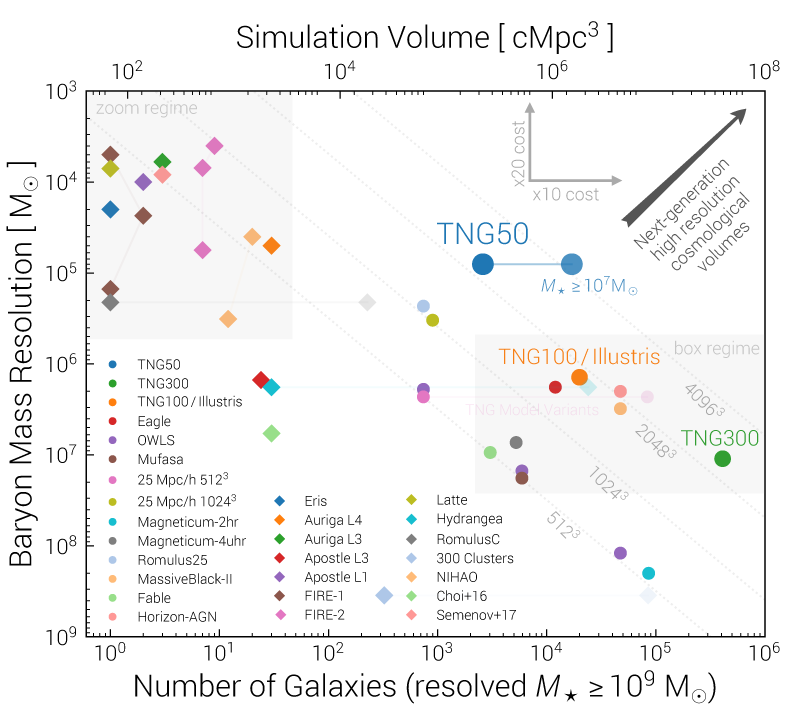
\includegraphics[width = \linewidth]{Figures/Chapter2/VolumeResolutionComparison.png}
    \caption{Image used with permission from: Illustris-TNG Project, \citet{Nelson2019FirstFeedback}}
    \label{fig:Vol_v_Res}
\end{figure}

In semi-analytic and semi-empirical models the analogous feature is found in the selection of merger trees fed to the models\footnote{For those semi-analytic/semi-empirical models that use n-body dark matter directly they follow the same pattern as the above but with dark matter particle resolution and number of haloes.} the number of haloes on a given merger tree is directly related to the lowest mass halo of interest. However, models using merger trees have one additional level of flexibility they can have a minimum subhalo mass and a minimum central halo mass. This provides flexibility in what can be simulated, for example:
\begin{itemize}
    \item High mass centrals, large box, high threshold for both central and subhalo mass. Suitable for exploring the evolution of massive galaxies.
    \item High mass centrals, medium/small box, low threshold for subhalo masses, moderate/high threshold for central masses. Suitable for exploring the environments around massive galaxies.
    \item Moderate/low mass centrals, medium/small box, low threshold for centrals and subhaloes. Suitable for exploring the evolution of large populations of smaller galaxies.
\end{itemize}


\steel has been specifically designed to not suffer from this trade-off by using a \textit{'Statistical Dark Matter Accretion history`} described in full in Section \ref{subsec:SDMAH}. In brief, the statistical accretion histories follow the average growth of a given mass of halo backwards in time from $z = 0$. At each time-step the USHMF is assigned to the halo mass track by comparing the USHMF at t and t +$\Delta$t the subhalo accretion in $\Delta$t is calculated. The lifetime subhaloes is assigned using dynamical time arguments. This accretion history requires only the average halo mass tracks and the SHMF, each of which is a numerical quantity for each mass bin one mass track is calculated and scatter is implemented using the intrinsic statistical distributions of galaxies where appropriate. \steel therefore simulates massive haloes and small haloes equally and is able to produce massive rare galaxies in the same run as smaller galaxies whilst simulating neither with higher precedence.

\subsection{Flexibility through stability}
%Flexibility - empirical
Hydrodynamical and Semi-Analytic models are tuned for two reasons. The first is for stability, these models have tens of parameters acting in the sub-grid for hydrodynamical or as the primary modelling tool for semi-analytic models. The issue stems from multiple parameters contributing to one galaxy variable, changing one parameter ripples throughout the model. In abstract consider a model with two parameters, $\alpha$ that controls a galaxy mass with a secondary effect on size, and $\beta$ that controls galaxy colour with a secondary effect on galaxy mass. Changing $\beta$ with the intent of modifying the colour of galaxies will force a reaction in $\alpha$ to compensate for the change in mass and then propagate into the size of galaxies. Secondly, the tuning allows fits to observations, the models are given freedom in their parameter sets to fit many galaxy properties at the same time but due to the overlap in what each physical assumption can control this leads to degeneracy in parameter space. To complicate comparison further, some models have more physical routines than others resulting in models and parameters in the less complex model compensating for this missing physics. The diversity in models and the diversity introduced by different tuning data has been extensively discussed in the literature \cite{Knebe2015NIFTyModels,Cui2018TheApplications,Knebe2018CosmicModels}.   

This degeneracy has in some part been addressed by semi-empirical models. Fundamental variables such as galaxy stellar mass are set using techniques such as abundance matching (Section \ref{C2:SubSec:AbnMtch}), doing so removes the reliance on the physical models and parameters that are required to tune to this quantity. 'Bottom-up' modelling like this gives semi-empirical models the ability to use dramatically reduced parameter spaces and then reproduce essential observable such as the central stellar mass function by design. Additional physical models are added only where necessary creating tight constraints for the core of the model. Empirical modelling is reproducing the core structures and evolution
by design once stability has been achieved additions can be made in a modular fashion, for example in \citet{Shankar2014} with abundance matching constraining the growth of galaxies and the halo structures the merger histories a size evolution model can be independently invoked. Semi-empirical models can use this to massive advantage testing, for example, multiple size evolution models on one assembly background without need for re-tuning or fear of disrupting the essential results. In this thesis we extend this idea of empirical stability and flexibility further, using the statistical backbone as discussed physical models are turned into probabilistic models that cannot influence the central galaxy growth. These models are entirely modular and can be added or removed at will and there impact on the populations can be individually analysed. 

It is noteworthy that some hydrodynamical cluster simulations are now able to use a technique with "genetically modified" haloes/galaxies by running a simulation multiple times and making slight adjustments they can do an 'apples to pears' comparison. This vernacular has the intended meaning that the models are nearly the same for example changing the distribution of dark matter without changing the total mass can change the merger mass ratios of galaxies and such look at how the merger mass ratio affects the final galaxy in two near-identical systems. This is a highly complementary and powerful technique that is yet to be fully realised \cite{Rey2018QuadraticHistory}.

\subsection{Consistency}
%Consistency - ensuring connections between high and low redshift
It is well documented that reproduction of the stellar mass function as multiple epochs has been a challenge for semi-analytic models \cite{Knebe2018CosmicModels, Asquith2018CosmicModels} and hydrodynamical models (although major improvements have been seen recently, for example, Illustris vs Illustris TNG \cite{Nelson2015TheRelease, Nelson2018TheRelease}). This has not however prevented such models from making bold claims about the successes of their models in terms of morphology and mass assembly without providing a full stellar mass function history \cite[e.g.][]{Somerville2008ANuclei, Hopkins2010MERGERSMATTER}\footnote{A merger history matched to an observational merger history as provided by \citet{Hopkins2010MERGERSMATTER} is insufficient as we show in Chapter \ref{Chapter:GalPairs} the methods involving pair fractions used to estimate these rates have a large degree of systematic error.}. However, it is the opinion held by PG that these claims should be viewed as entirely unsubstantiated. As an example, if a kettle at temperature A that is modelled to cool under an arbitrary physical model $\gamma$ to temperature B in time T. If A is observed to be false compared to the data and B is observed to be consistent with the data than the inference that $\gamma$ is a correct physical model is baseless. Galaxy models that fail to reproduce the stellar mass function at high redshift repeatedly invoke this kind of logic when the z=0 stellar mass function is reproduced. An overabundant stellar mass function at high redshift that evolves to the observed stellar mass function at low redshift implies either lack of growth in the galaxy population to allow the observed stellar mass function to catch up or over merging of galaxies to reduce the total number density.

A semi-empirical model that puts reproduction of the stellar mass function and the distribution of satellite galaxies as the foremost modelling priority has a major advantage. Any internally self-consistent model is a viable candidate for the true physical model with stronger evidence than those presented in models that do not achieve consistency over multiple epochs. 

\subsection{Speed}
%Systematics - speed

Speed is a critical ingredient to any model, hydrodynamic models have run-times of months using millions of CPU hours, and semi-analytic models constrain highly-multi dimensional parameter space for thousands of merger histories. In each case speed allows for the models to reach conclusions in shorter time frames. Semi-empirical models are faster by design with smaller better-constrained parameter spaces, they can therefore leverage more computational time to explore physical models or larger simulation boxes. In forgoing discrete merger trees the run time of \steel depends on different factors to other models, the width of the mass bins used for the halo and subhalo mass functions (which corresponds to the resolution of halo or mass particle) and secondly is the computational complexity of any physical modelling routines. Where \steel is not running to tune to high N parameter space or thousands of discrete merger trees it can instead test combinations of internal physical models or be run on more modest, cheaper, and widely accessible hardware.

\section{Modules and Methods}

\subsection{Statistical Dark Matter Accretion History}
\label{subsec:SDMAH}

Undeniably the single most important element of \steel and a large part of what makes it unique and enables an alternative view of galaxy formation problems is the \textbf{\textit{statistical dark matter accretion history}}. As described above a large part of the power of \steel come from the removal of discrete merger tress or haloes achieved using this technique. We provide here a discussion of n body and processed merger trees building upon Section \label{sec:LCDM} followed by a detailed description of how the statistical dark matter accretion history is constructed.

%First we should explain merger trees and traditional simulation techniques.
\subsubsection{Traditional methods and merger trees}

%first n body

The state of the art in dark matter modelling is n-body simulations, simulating billions of individual particles and solving the equation of state for each over many epochs to simulate their evolution from the distributions calculated from the CMB to the cosmic web of haloes and filaments inferred from observations of galaxies today. The non-interacting nature of \textbf{cold} dark matter is extremely fortuitous as it means its behaviour can be modelled using gravitational tensors only thus modern dark matter simulations are able to leverage the massive power gains made recently in GPU computing allowing for ever larger and higher resolution dark matter only simulations to be run. 

Whilst the massive n-body simulations are impressive they do little to impact our understanding of galactic astrophysics, the outputs of even the previous generation n-body dark matter simulations such as the Bolshoi simulation a snapshot of which is shown in Figure \ref{fig:Bolshoi} total tens of gigabytes for individual sections and terabytes to capture the whole simulation. To use all of this information would be impractical for any galactic modeller without access to high-performance computing hardware and a good understanding of memory management. Furthermore despite the excellence provided by halo-finders and merger tree extractors such as \textsc{rockstar} \cite{Behroozi2013THECORES} and the consistent trees algorithm' \cite{Behroozi2013GRAVITATIONALLYCOSMOLOGY}, the merger trees are frequently not fit for use in models not specifically built to handle these inputs. Furthermore, as discussed by van den Bosch \cite{vandenBosch2014ComingWells, vandenBosch2017DissectingSimulation, vandenBosch2018DisruptionFiction} the interpretation of dark matter simulations is of vital importance, as the analysis tool and the fundamental design decisions taken in building the simulation all have systematic effects on the outputs all of which complicating comparison between simulation.

\begin{figure}[h]
    \centering
    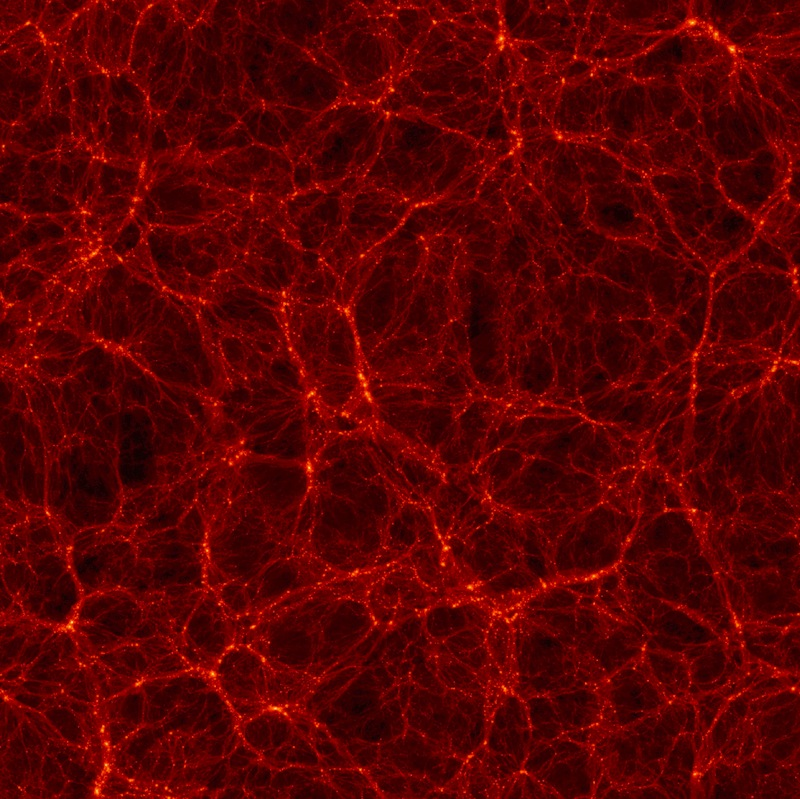
\includegraphics[width = \linewidth]{Figures/Chapter2/Bolshoi.jpg}
    \caption{Snapshot of the 250 Mpc$^3$ box of the Bolshoi Simulation. Brighter regions indicate a higher density of dark matter. Note the clustered bright points connected by large filaments. This structure is known as the cosmic web.
    Image credit: Bolshoi Simulation http://hipacc.ucsc.edu/Bolshoi/Images.html}
    \label{fig:Bolshoi}
\end{figure}

The choice of many analytic or empirical models to instead opt for analytically derived Press Schecter trees that can be generated 'on-the-fly' or pre-processed comes for the simplicity and flexibility afforded by this technique. However, trees generated in this way are still affected by volume (i.e. number simulated) and resolution (i.e. size of the smallest halo accounted for in any split) limiting there effectiveness.

\subsubsection{State of the art statistical method}
%then get onto what makes STEEL STEEL
\begin{figure}[h!]
    \centering
    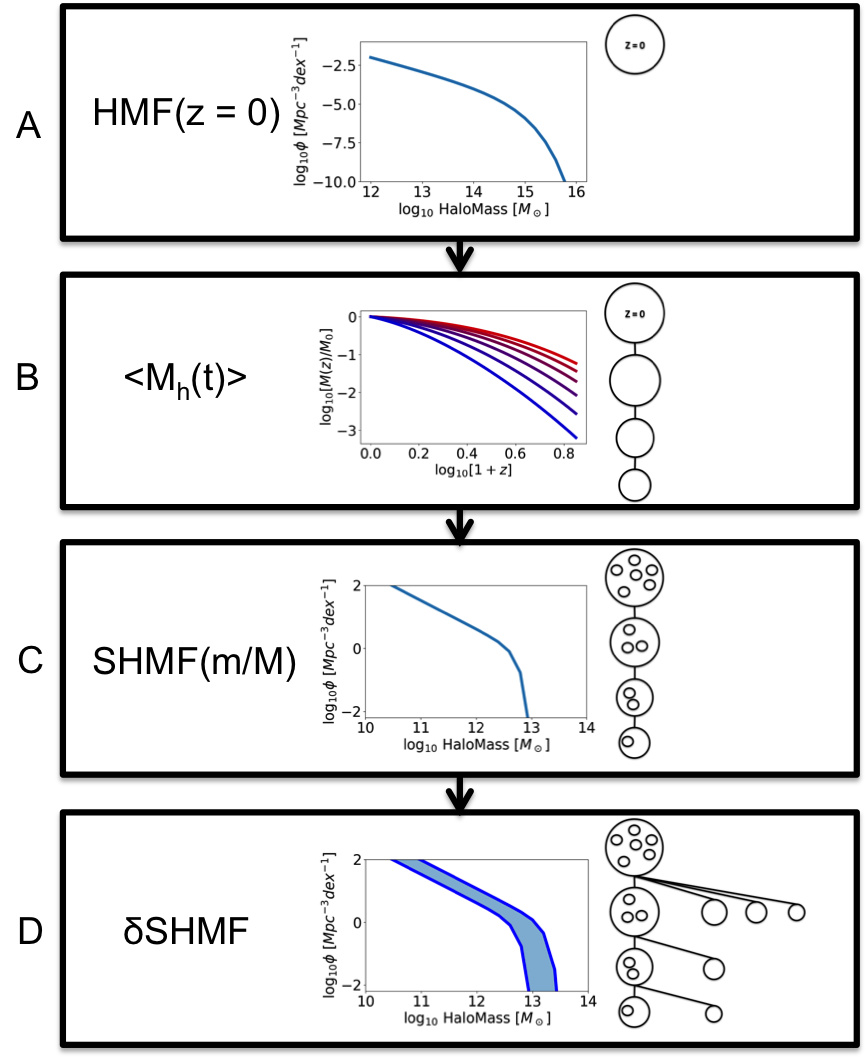
\includegraphics[width = \linewidth]{Figures/Chapter2/StatDM.png}
    \caption{We show the main steps in building the statistical dark matter accretion history for STEEL. Each panel shows a feature from a traditional merger tree and the statistical function used to replace it. A: The HMF is used to calculate the number densities of central haloes. B: Average mass growth histories are used to calculate the size of each mass bin at previous epochs. C: The (unevolved)SHMF is used to populate each central at each redshift with subhaloes. D: The average number densities of accreted subhaloes at each epoch are calculated by taking the difference between each mass bin of the (unevolved)SHMF at consecutive redshift steps.}
    \label{fig:StatDM}
\end{figure}


The core principle of the statistical methodology is to treat parent haloes, and satellites galaxies/haloes, as ``average'' populations avoiding issues with volume and resolution as described previously. Here we detail step by step construction of the statistical dark matter accretion history complemented with a graphic representation in Figure \ref{fig:StatDM}.

\textbf{Central Haloes}

We start by considering a fine grid of central dark matter haloes ranging from $M_{h}=10^{11}\, M_{\odot}$ to $M_{h}=10^{15}\, M_{\odot}$ at redshift $z=0$. Their number densities are given by the halo mass function (HMF) of \citet{Despali2016TheDefinitions}, which is obtained using the COLOSSUS Python package \citep{Diemer2017COLOSSUS:Halos} which contains many other halo mass functions as well as spherical overdensity conversions required throughout this work. 

The halo mass function provides the number of densities of haloes in a given mass bin (Figure \ref{fig:StatDM}, Panel A).
The average mass growth histories of all main progenitors with mass in the bin of halo mass $[M_{h},M_{h}+dM_{h}]$, are then calculated using the analytic model from \cite{vandenBosch2014ComingWells}\footnote{This model further improves on the seminal work by \citet{Parkinson2008GeneratingTrees}, which was aimed at reproducing numerical merger trees, optimized with small redshift steps minimizing the development of systematic errors at late cosmic epochs.}. This provides the average ``main progenitor'' branch of a traditional merger tree for each mass bin at $z = 0$ (Figure \ref{fig:StatDM}, Panel B.)

\textbf{Assigning Subhaloes to Parent Haloes}

In order to predict the number of satellite galaxies, we must associate to each parent/central halo the number and mass of subhaloes they are expected to contain. To achieve this we use the subhalo mass function (SHMF). The SHMF describes the expected distribution of subhaloes, of mass $M_{h,sat}$, in a given parent halo of mass $M_{h,cent}$, as a function of $M_{h,sat}/M_{h,cent}$. Multiple definitions for the SHMF exist depending on the way a subhalo is defined. In this work we use two definitions of the SHMF. The first is the unevolved SHMF (USHMF), which describes the total subhaloes accreted over a parent halo's lifetime. In the unevolved SHMF any merging or stripping in the subhaloes occurring after infall is ignored. Several groups have been able to constrain the unevolved SHMF \citep{Giocoli2008AnalyticalHaloes,Jiang2016StatisticsFunctions}. In what follows, we use the latest rendition of the unevolved SHMF by \citet{Jiang2016StatisticsFunctions}, which is calibrated against the Bolshoi simulation\footnote{ We direct the interested reader to \citet{Jiang2016StatisticsFunctions} for further discussion of the unevolved SHMF as well as of other SHMFs, such as the evolved SHMF where the number densities are affected by both subhalo stripping and mergers.}.

The second definition we use in this work is the unevolved ``surviving'' SHMF (USSHMF). Subhalo masses are assumed frozen at infall but the subhalo number densities can reduce compared to the unevolved SHMF as the unevolved surviving SHMF accounts for subhalo disappearance due to tidal disruption in the parent halo. We show in Figure \ref{fig:SHMF_clus} for a representative parent halo of mass $\log M_{h,cent} M_{\odot} = 12.80$, the unevolved SHMF and three unevolved surviving SHMF characterized by different dynamical friction timescales $\tau_{dyn}$. Larger $\tau_{dyn}$ lead to a milder reduction in subhalo number densities as subhaloes take longer to merge with the parent halo. Lower $\tau_{dyn}$ are less effective in reducing the number densities of smaller subhaloes which are more likely to have dynamical friction timescales comparable to or larger than the Hubble time at $z = 0$.
\begin{figure}[h!]
    \centering
    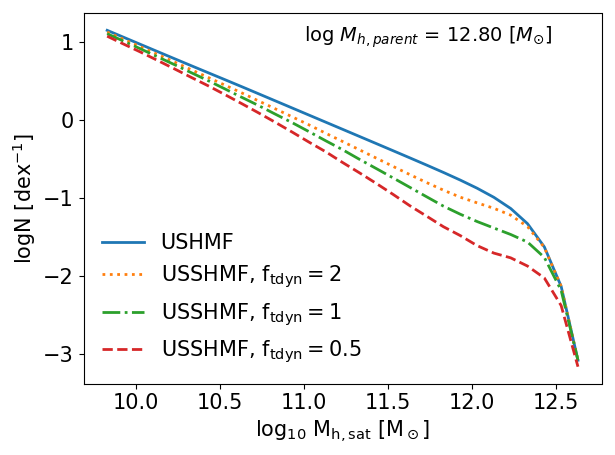
\includegraphics[width = \linewidth]{Figures/Chapter2/SHMF_OneCluster.png}
    \caption{Comparison between the unevolved SHMF (solid line) and three unevolved surviving SHMF  (dotted lines) for a parent halo of mass $\log$ $M_{h,parent}$ $[M_{\odot}] = 12.80$. The factor $f_{t_{dyn}}$ is applied to the merging timescales of the haloes. Lower factors correspond to lower unevolved surviving SHMF where more sub haloes have merged.}
    \label{fig:SHMF_clus}
\end{figure}

\textbf{Average Subhalo Accretion}

At each redshift step along with the mass growth histories, we calculate the unevolved SHMF associated to the parent halo mass. This is equivalent to the substructure found in traditional merger trees (Figure \ref{fig:StatDM}, Panel C). However, unlike traditional methods, our statistical approach is able to probe ``rare'' subhaloes without running prohibitively large volumes of merger trees.

For each time step we can now calculate a mass function describing the number density of subhaloes accreted onto the population of central haloes in the halo mass bin $[M_{h,cent}(z),$ $M_{h,cent}(z) + dM_{h,cent}(z)]$. The latter is achieved by differentiating the unevolved SHMF across two neighbouring redshift steps $z$ and $z+dz$, we can calculate the average number density of subhaloes of any given mass $M_{h, sat}$ that are accreted in the redshift interval $dz$ onto the main progenitor haloes with mass in the bin $[M_{h,cent}(z),$ $M_{h,cent}(z) + dM_{h,cent}(z)]$,
\begin{equation}
\label{eqn:deltSHMF}
\begin{split}
&\delta USHMF[z, M_{h,cent},M_{h,sat}] =  \\
&USHMF\Big(\frac{M_{h,sat}}{M_{h,cent}(z)}\Big) - USHMF\Big(\frac{M_{h,sat}}{M_{h,cent}(z + \delta z)}\Big)
\end{split}
\end{equation}
In this way the unevolved subhalo accretion history ($\delta USHMF$) is retrieved for all main progenitor haloes at all redshifts.


\subsection{Abundance matching}
\label{C2:SubSec:AbnMtch}
In this work we populate dark matter haloes with galaxies using the abundance matching technique where galaxies are assigned to haloes by comparing the relative abundances of galaxies and haloes. For example in Figure \ref{fig:Abn_Toon} the horizontal lines connect points of constant number density between the HMF (red, top left) and the SMF (green, bottom right). Halo/stellar masses with corresponding number density are then define a mapping between the masses called the stellar-mass-halo-mass (SMHM) relationship (black, bottom left).

\begin{figure}[h]
    \centering
    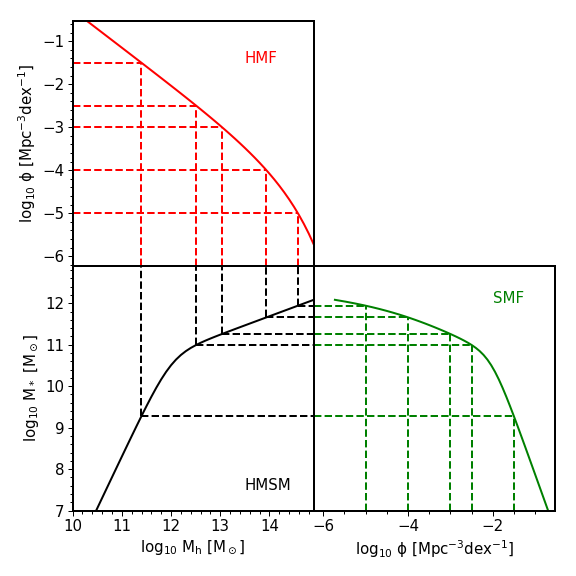
\includegraphics[width = \linewidth]{Figures/Chapter2/AbundaceMatching.png}
    \caption{A cartoon to show by matching the HMF (top left) and the SMF (bottom right) by abundance and the mapping between stellar and halo mass referred to as a SMHM relation (bottom left) is created.}
    \label{fig:Abn_Toon}
\end{figure}

The abundance matching used in \steel takes central haloes from the halo mass function from \citet{Despali2016TheDefinitions} obtained using \textsc{colossus}\cite{Diemer2017COLOSSUS:Halos}, and a subhalo mass function subdivided by the redshift of infall generated from the statistical dark matter accretion history used by \textsc{steel}. Subhaloes are assumed to follow the central SMHM relation at infall. We simplify our abundance matching by using a frozen model such that baryonic evolution after infall (stripping, star formation, etc.) is not included. The latter assumption provides a good approximation as after infall the dominant factor determining the abundances of satellite galaxies is the dynamical time and not evolutionary processes (Paper \RomanNumeralCaps{1}).

To fit stellar mass functions over multiple epochs we convolve our halo mass functions with a parametric SMHM relation similar to that proposed by \cite{Moster2010},
\begin{equation}
\label{eqn:MosAbn}
\begin{split}
M_*(M_h, z) &= 2M_hN(z)\Big[ \Big( \frac{M_h}{M_{n}(z)}\Big) ^{- \beta(z)} + \Big( \frac{M_h}{M_{n}(z)}\Big)^{\gamma(z)} \Big ]^{-1}\\
N(z) &= N_{0.1} +N_z\Big(\frac{z-0.1}{z+1}\Big)\\
M_{n}(z) &= M_{n,0.1} +M_{n,z}\Big(\frac{z-0.1}{z+1}\Big)\\
\beta(z) &= \beta_{0.1} +\beta_z\Big(\frac{z-0.1}{z+1}\Big)\\
\gamma(z) &= \gamma_{0.1} +\gamma_z\Big(\frac{z-0.1}{z+1}\Big).
\end{split}
\end{equation}

In what follows we adopt both the cmodel and PyMorph SMF described in Section \ref{subsec:SMF} at redshift $z=0$ to constrain the parameters N, M, $\beta$, and $\gamma$ (normalization, knee, low mass slope, and high mass slope). We use only the central stellar mass function, using the \cite{Yang2012EvolutionHalos} central/satellite identification, and central halo mass function. The fit is performed using a Markov Chain Monte Carlo (MCMC), implemented using the \textsc{python} package \textsc{emcee} \citep{Foreman-Mackey2013Emcee:Hammer}, over a large parameter space ($P_{M, N, \beta, \gamma}$) covering all four parameters. Given a point in parameter space $P_{M_i, N_i, \beta_i, \gamma_i}$, the stellar mass function is constructed using the halo mass function and the SMHM relation. Each bin of parent halo mass is associated with a Gaussian distribution of stellar mass with scatter 0.15 dex. This distribution is multiplied by the halo mass number density to convert to galaxy number density which is added to the relevant stellar mass bins of the stellar mass function in construction. This operation is then repeated overall mass bins of the halo mass function to produce the complete central stellar mass function. For each point, $P_{M_i, N_i, \beta_i, \gamma_i}$ in the parameter space, the stellar mass function associated to that point is compared via a likelihood function to the observed stellar mass function to provide the MCMC with the probability that the given point is the `true' SMHM relationship. 

We then fit to the \cite{Davidzon2017TheSnapshots} data both uncorrected and corrected for the cmodel and PyMorph fits respectively (see Section \ref{subsec:SMF} for details). At high redshift we use the central and subhalo mass functions initializing satellites at infall as described above\footnote{Ideally, as for low redshift, we would use the centrals only as we are primarily concerned with the central SMHM relation. However, lacking a well-defined central stellar mass function at high redshift, this method represents a reliable way to extend the model to higher redshifts.}. For central haloes the method is the same as detailed above, however, as we use the total stellar mass functions at high redshift we also include the total unevolved surviving subhalo mass function in the abundance matching. 
We assume that a halo before infall hosts a central galaxy; under this assumption we use the central SMHM relation to assign satellite galaxy stellar mass at the point of accretion. For the latter, we must have information about the redshift of infall for subhaloes. We obtain from \textsc{steel} the unevolved surviving subhalo mass function as contributed by each redshift of infall. Each contributing part is calculated using the SMHM relation at the redshift of infall and added to the central stellar mass function using the same method as with the centrals. The total stellar mass function is compared, at each redshift step available, to the data via the likely-hood function to give the probability that the given point is the `true' evolution parameters. The abundance matching best-fit parameters and associated errors for both the cmodel and PyMorph are given in Table \ref{tab:AbnResult}, and plots showing the cross-sections of the parameter space are shown in Appendix \ref{Appx:AbnMCMC}.

\begin{table}
\centering
\begin{tabular}{l|llllllll}
        & M\_n & N     & $\beta$ & $\gamma$ & $M_{n,z}$ & N\_z   & $\beta_z$ & $\gamma_z$ \\ \hline
\\
cmodel  & $11.91_{-0.34}^{+0.40}$ & $0.029_{-0.013}^{+0.018}$ & $2.09_{-1.02}^{+1.21}$    & $0.64_{-0.10}^{+0.11}$     & $0.52_{-0.19}^{+0.24}$       & $-0.018_{-0.004}^{+0.005}$ & $-1.03_{-0.34}^{+0.049}$     & $0.084_{-0.14}^{+0.20}$      \\
\\
PyMorph & $11.92_{-0.36}^{+0.39}$ & $0.032_{-0.012}^{+0.016}$ & $1.64_{-0.73}^{+0.85}$     & $0.53_{-0.11}^{+0.11}$     & $0.58_{0.19}^{+0.15}$        & $-0.014_{-0.006}^{+0.007}$ & $-0.69_{-0.36}^{+0.29}$      & $0.03_{-0.147}^{+0.154}$      
\end{tabular}
\caption{The abundance matching results for the cmodel and PyMorph data. The errors are the 16th and 86th percentile from the MCMC fiting.}
\label{tab:AbnResult}
\end{table}

\begin{figure}[h]
    \centering
    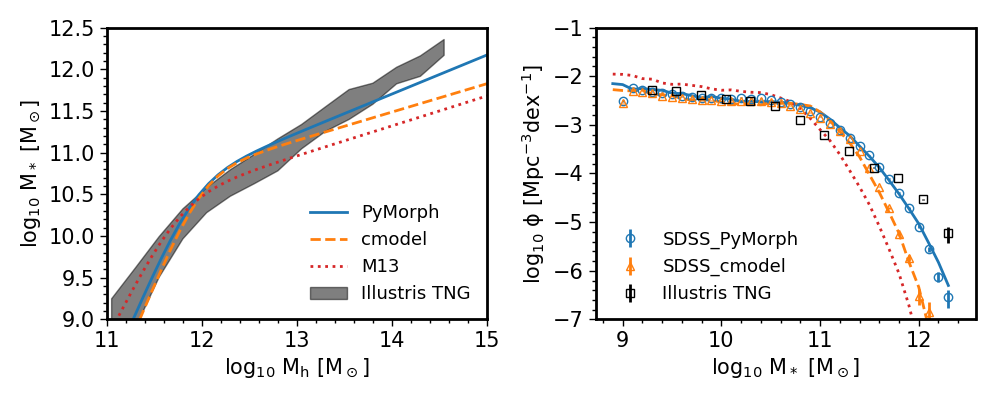
\includegraphics[width = \linewidth]{Figures/Chapter2/AbundaceMtch_Data.png}
    \caption{Left: The SMHM relation at redshift $z=0.1$. The PyMorph (blue solid line) and cmodel (orange dashed line) fits from this work are both for central haloes/galaxies, the fit from \citet{Moster2013} (M13, red dotted line) is for all haloes/galaxies. The grey band is the relation from Illustris TNG100. Right: Stellar mass functions created using the central halo mass function and the three SMHM relations compared to PyMorph (blue circles) and cmodel (orange triangles) central stellar mass functions. The black squares are the stellar mass function from Illustris TNG100.}
    \label{fig:Abn_Data}
\end{figure}

In Figure \ref{fig:Abn_Data} we show the results of our abundance matching to the PyMorph and cmodel central stellar mass functions. The PyMorph fit is steeper above the knee compared to either the cmodel or the \citet{Moster2013} model fits, as expected given the larger number density of massive galaxies found applying the S\'ersic-Exponential model \citep[eg.,][]{Shankar2014, Kravtsov2018StellarHalos}. The low mass slope for both PyMorph and cmodel are almost identical as the galaxies in this range are not affected by the photometric choice. Differences between the fits from this work and \citet{Moster2013} are due to our selection of using only central haloes/galaxies as opposed to the total population, and the stellar mass functions shown in the right-hand panel are lower than even cmodel are therefore missing massive galaxies.


\subsection{Continuity star formation rate}

The continuity star formation rate was theorised in an effort to reconcile the observed evolution of the stellar mass function and the observed star formation rate. The observed UV star formation rates applied to high redshift stellar mass functions evolving populations conserving number density yield stellar mass functions higher than those observed. This deviation proved challenging for models which can not simultaneously reproduce the observed SFR and SMF, without invoking harsh feedback routines.

\begin{figure}[h]
    \centering
    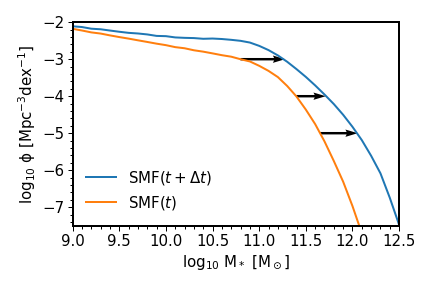
\includegraphics[width = \linewidth]{Figures/Chapter2/ContinuityEqn.png}
    \caption{The continuity approach connects at constant number density galaxy populations across cosmic time. Between two epochs `$t$' and `$t + \Delta t$' the SMF grows differently at different number density. The mass difference, $\Delta M$, indicated at three number densities by black arrows is the expected mass growth for each population.}
    \label{fig:Cont_Eqn}
\end{figure}

The continuity star formation rate is a theoretical quantity calculated such that the observed growth of the stellar mass function is conserved. As illustrated in Figure \ref{fig:Cont_Eqn} by connecting two SMF at consistent number density at times `$t$' and `$t + \Delta t$' the growth in mass $\Delta M$ at each number density over the time $\Delta t$ is obtained. In the simplest approximation, the SFR is equal to $\Delta M / \Delta t$. However, the star formation rate is higher than the this value. As new stars are created a proportion of the mass is recycled through supernova 'quickly' in terms of cosmological time. This mass recycling given in \citet{Moster2018Emerge10} is used to amend the star formation rate, to account for the mass loss based on the entire star formation history of the galaxy. The fraction of mass lost by a population of stars over time $\tau_{ml}$ is given by,

%Mass recycling
\begin{equation}
\label{eqn:f_ml}
f(\tau_{ml}) = 0.05 \ln \Big(\frac{\tau_{ml}}{1.4 Myr}+1\Big) ,
\end{equation}

summing the difference in fraction lost in a time step $\delta t$ for every star formation epoch in the galaxies history (SFH) gives the mass loss rate (MLR), 

\begin{equation}
\label{eqn:MLR}
MLR(t) = \frac{ \sum_{t' = t_{inf}}^{t} SFH(t')(f[t' - (t-\delta t)]-f[t' - t]) }{\delta t} .
\end{equation}

The continuity SFR is therefore calculated to be $\Delta M / \Delta t$ + MLR. The final correction made to this star-formation rate is that galaxies also accrete mass via mergers this accrete mass term ($M_{acc}$) is prominent for massive galaxies $M_* > 10^{11} M_{\odot}$. The continuity SFR at time t' is then finally,

\begin{equation}
    SFR_{continuity}(t') = \frac{\Delta M(t')}{\Delta t} + MLR(t') - M_{acc}(t').
\end{equation}

\subsection{Empirical central galaxy growth}

Using the stellar-mass-halo-mass (SMHM) relation and halo mass growth histories (HMGH) we make an empirical prediction of the average central galaxy growth. In Figure \ref{fig:Cent_Mass_PP} we show in the top left the HMGH for two haloes $M_{z=0} = 10^{14}, 10^{12.5} M_{\odot}$, the middle panel shows the SMHM where the shading shows the extent of the evolution of the median of the relation over the redshift range, finally the bottom left shows the stellar mass growth history (SMGH) predicted by the latter two inputs.

%include a plot of using AM to convert HMGH to SMGH?
\begin{figure}[h]
    \centering
    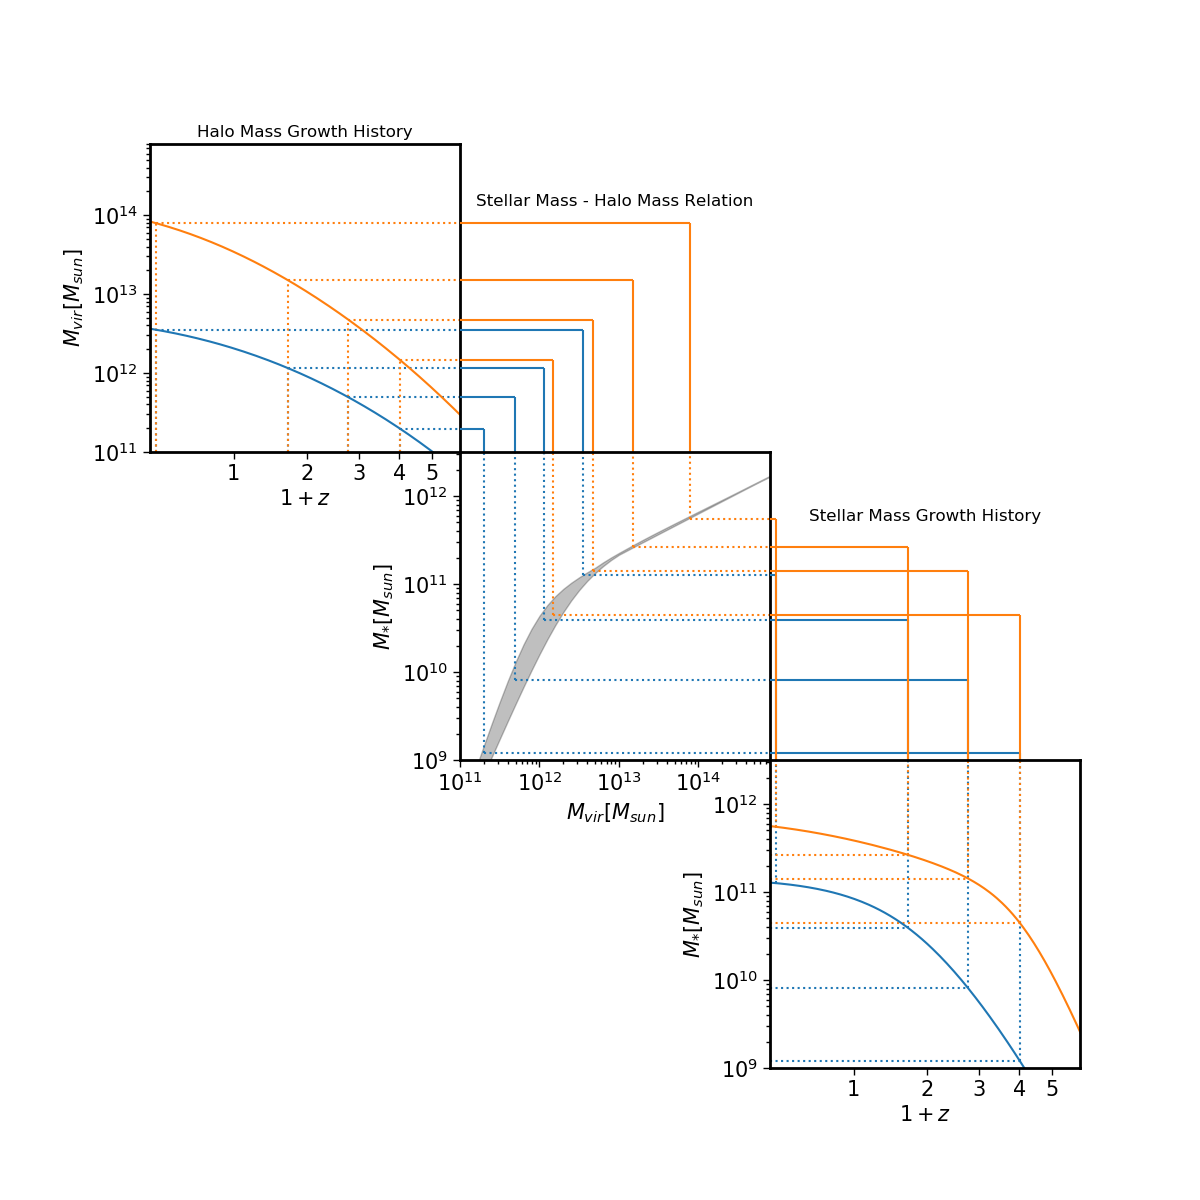
\includegraphics[width = \linewidth]{Figures/Chapter2/HMGH_to_SMGH.png}
    \caption{The Halo Mass Growth Histories (HMGH, top-left) are propagated through the redshift dependent stellar-mass-halo-mass relation (SMHM, middle) to produce corresponding Stellar Mass Growth Histories (SMGH, bottom-right). The lines illustrate matching points in redshift and the intersection with the SMHM relationship. The width of the SMHM relationship shows the extent of evolution with time, not as is common the scatter.}
    \label{fig:Cent_Mass_PP}
\end{figure}

At several redshift epochs, the HMGH to the SMGH are connected following the colour-coded lines, it is found the shape of the SMHM relationship is the primary factor that dictates the shape of the SMGH. Identifying for each growth history the step before the central galaxy growth rapidly slows z = 3 for orange and z = 1 for blue each of these lines intersect the HMGH when it is still growing, whereas they intersect the SMHM relationship just before the 'knee'. This change in the growth behaviour is thought to be an effect of active galactic nuclei suppressing the formation of stars in a galaxy. However, as the knee is a function of halo mass once could also attribute this to the halo mass at which infalling gas is shock heater and can no longer efficiently accrete to the central galaxy.

\section{Discussion}
